\documentclass[12pt]{article}
\usepackage[top=1in, bottom=1in, left=1.25in, right=1in]{geometry}
\usepackage{iftex}
\usepackage{graphicx}
\usepackage{enumitem}
\usepackage{xr-hyper}
\usepackage{hyperref}
%\externaldocument{appendix3}
\renewcommand{\figureautorefname}{Fig.}
\usepackage[utf8]{inputenc}
\usepackage{newunicodechar}
\newunicodechar{α}{$\alpha$}
\newunicodechar{β}{$\beta$}
\newunicodechar{γ}{$\gamma$}
\usepackage[style=apa, backend=biber]{biblatex}
\addbibresource{fvpollens.bib}
\setcounter{maxnames}{20}
\setcounter{minnames}{1}
\usepackage{color}
\usepackage{amsmath}
\usepackage{amssymb}
\usepackage[export]{adjustbox}
\usepackage{verbatim}
\usepackage{mathpazo}
\usepackage{setspace}
\usepackage{multirow}
\usepackage{lscape}
\usepackage{fancyhdr}
\usepackage[normalem]{ulem}
\usepackage{rotating}
\usepackage{chngcntr}
\usepackage[parfill]{parskip}
\usepackage[tiny,compact]{titlesec}
\usepackage{longtable}
\usepackage{textcomp}
\usepackage{rotating}
\usepackage{xr}
\usepackage{caption}
\usepackage{booktabs}
\usepackage{siunitx}
\usepackage[T1]{fontenc}
\usepackage{gensymb}
\usepackage{float}
\captionsetup{font=footnotesize}
\sisetup{round-mode=places, round-precision=2, detect-all}
\hypersetup{colorlinks=true, linkcolor=black, citecolor=black}
\RequirePackage{lineno}

\def\title{Appendix for ``Bumblebees like flowers...presumably?''}

\def\author{Jenna B. Melanson$^{1*}$, Natalia Clermont$^{2}$, Tyler T. Kelly$^{2}$, Claire Kremen$^{1,2}$}



\clearpage
\def\affiliation{
  \begin{enumerate}
  \item Biodiversity Research Center, University of British Columbia, 2212 Main Mall, Vancouver, BC, Canada, V6T 1Z4
  \item Institute for Resources, Environment, and Sustainability, University of British Columbia, 2202 Main Mall, Vancouver, BC, Canada, V6T 1Z4
  \end{enumerate}
}

\def\runninghead{Bumblebee pollens}

\def\corr{\noindent
  $\star$ Corresponding author: Jenna B. Melanson (jenna.melanson@ubc.ca) \\
  \\
  }

\newcommand{\mstitlepage}{
  \paragraph{Running head:} \textsc{\runninghead}
  \parindent=0pt
  \begin{center}
    {\LARGE \title \par}
    \vskip 3em
    {\large
      \vspace{-20pt}
      \begin{tabular}[t]{c}
        \author
      \end{tabular}\par}
    \vskip 1.5em
  \end{center}\par
  \affiliation
}

\begin{document}
\mstitlepage
\doublespacing
\linenumbers
\renewcommand{\thesection}{A\arabic{section}}
\renewcommand{\thefigure}{A\arabic{figure}}
\renewcommand{\thetable}{A\arabic{table}}
\setcounter{figure}{0}
\setcounter{table}{0}
\setcounter{page}{1}
\clearpage

\section{Additional Figures}

\begin{figure}[H]
    \centering
    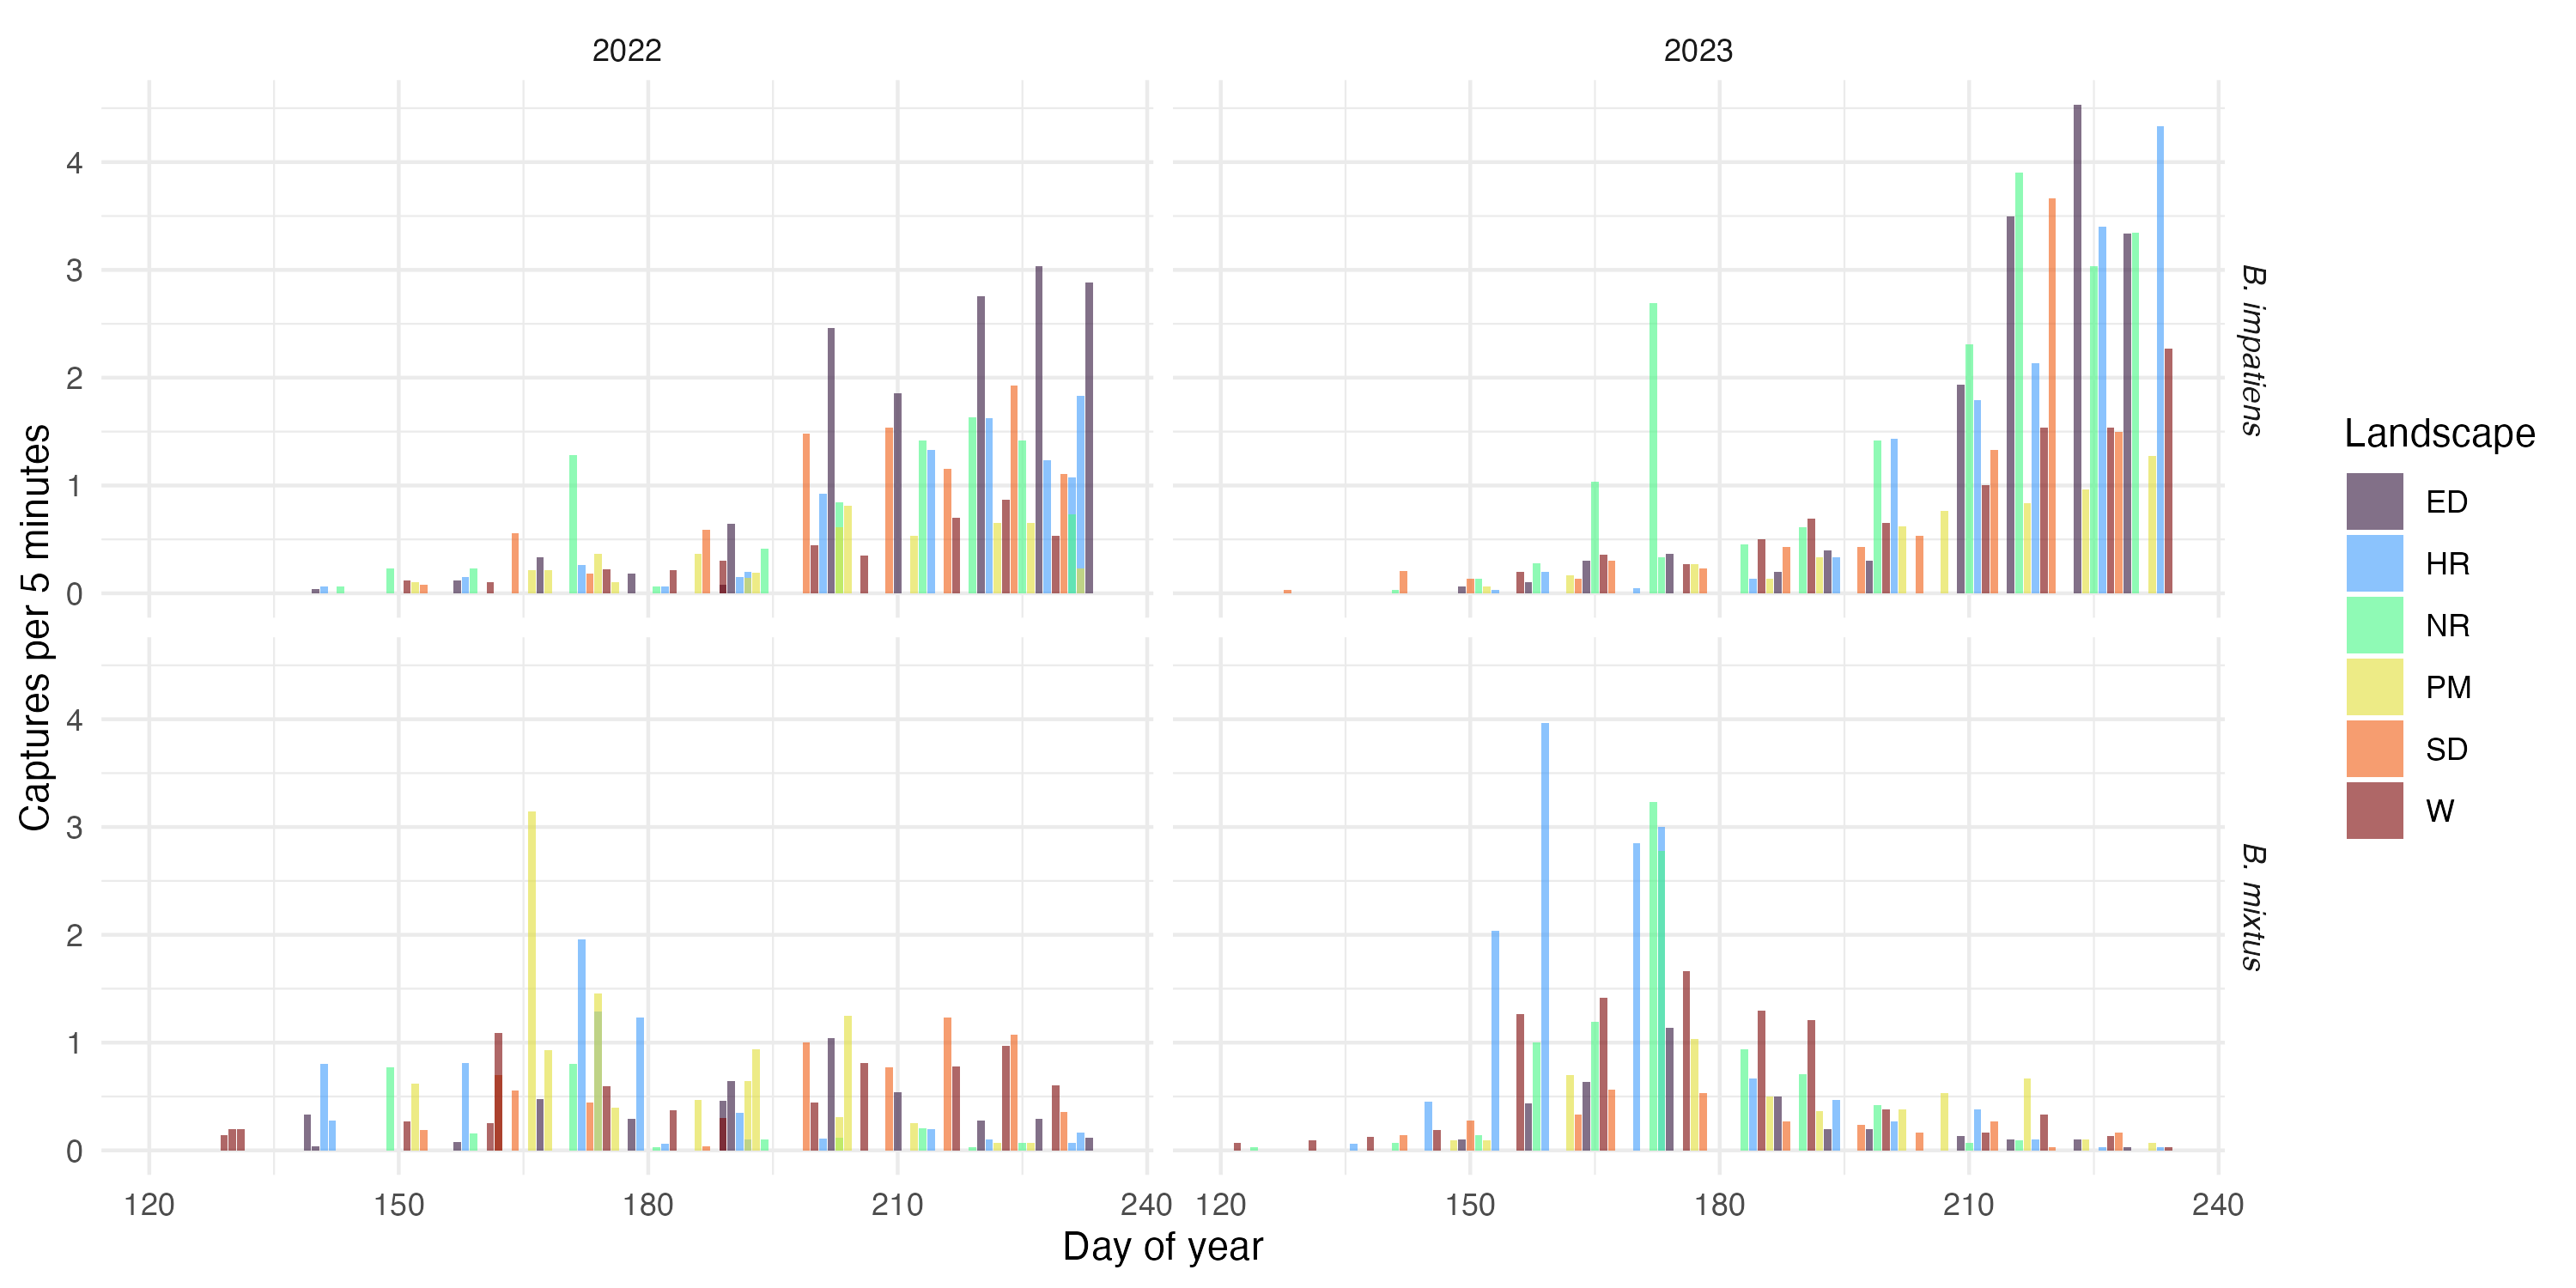
\includegraphics[width=\linewidth]{../7_figures/appendix_figures/speciesphenology.png}
    \caption{Worker phenology for \emph{B. mixtus} and \emph{B. impatiens} in 2022 and 2023. Bars are coloured by landscape; values are the total number of captures at a landscape on a given day, divided by the total number of (5 minute) sampling events conducted on that day. All available \emph{B. mixtus} pollen loads were sequenced; \emph{B. impatiens} pollen loads were sequenced for a subset of individuals captured between 18 July-16 August (i.e., day of year 199-228).}
    \label{fig:speciesphenology}
\end{figure}

\end{document}